% This is samplepaper.tex, a sample chapter demonstrating the
% LLNCS macro package for Springer Computer Science proceedings;
% Version 2.21 of 2022/01/12
%
\documentclass[conference]{IEEEtran}
%
\usepackage{xurl}
\usepackage[T1]{fontenc}
% T1 fonts will be used to generate the final print and online PDFs,
% so please use T1 fonts in your manuscript whenever possible.
% Other font encondings may result in incorrect characters.
%
\usepackage[pdftex]{graphicx}
% Used for displaying a sample figure. If possible, figure files should
% be included in EPS format.
%
% If you use the hyperref package, please uncomment the following two lines
% to display URLs in blue roman font according to Springer's eBook style:
%\usepackage{color}
%\renewcommand\UrlFont{\color{blue}\rmfamily}
%\urlstyle{rm}
%

%%%--------------------for using acronyms and generating a list of acronyms

\usepackage[printonlyused]{acronym}
\usepackage[toc,acronym,nomain,shortcuts,nonumberlist]{glossaries}
\usepackage{xcolor}
\usepackage{tikz}
\usepackage{url}
\usepackage{hyperref}
\makeglossaries
\newacronym{DOM}{DOM}{Document Object Model}
\newacronym{EVM}{EVM}{Ethereum Virtual Machine}
\newacronym{URL}{URL}{Uniform Resource Locator}
\newacronym{RPC}{RPC}{Remote Procedure Call} %%file that has all the acronyms
\renewcommand*{\acronymname}{List of Acronyms} %change the acronyms title while using printglossaries
%---------------------------------------------------------------------------------------------------------------------------------------------------

\definecolor{tone}{RGB}{255, 230, 204} %\textcolor{T1}{(1)}
\definecolor{ttwo}{RGB}{238, 238, 238}
\definecolor{tthree}{RGB}{250, 217, 213} % rgb(250 217 213)
\definecolor{tfour}{RGB}{213, 232, 212}

\newcommand\TONE[1]{%
  \tikz[baseline=(X.base)] 
    \node (X) [draw, shape=circle, inner sep=-1, fill=tone, minimum width=1em, text=black] {\strut #1};%
}
\newcommand\TTWO[1]{%
  \tikz[baseline=(X.base)] 
    \node (X) [draw, shape=circle, inner sep=-1, fill=ttwo, minimum width=1em, text=black] {\strut #1};%
}
\newcommand\TTWODASHED[1]{%
  \tikz[baseline=(X.base)] 
    \node (X) [draw, shape=circle,dashed, inner sep=-1, minimum width=1em, fill=ttwo, text=black] {\strut #1};%
}
\newcommand\TTHREE[1]{%
  \tikz[baseline=(X.base)] 
    \node (X) [draw, shape=circle, inner sep=-1, fill=tthree, minimum width=1em, text=black] {\strut #1};%
}
\newcommand\TTHREEDASHED[1]{%
  \tikz[baseline=(X.base)] 
    \node (X) [draw, shape=circle,dashed, inner sep=-1, fill=tthree, minimum width=1em, text=black] {\strut #1};%
}
\newcommand\TFOUR[1]{%
  \tikz[baseline=(X.base)] 
    \node (X) [draw, shape=circle, inner sep=-1, fill=tfour, minimum width=1em, text=black] {\strut #1};%
}
\newcommand\TFOURDASHED[1]{%
  \tikz[baseline=(X.base)] 
    \node (X) [draw, shape=circle,dashed, inner sep=-1, fill=tfour, minimum width=1em, text=black] {\strut #1};%
}

% = = = = = = = 
% Nuclear option if paper does not fit in page limit
%\usepackage[all=normal,paragraphs=tight]{savetrees}


\begin{document}
%
\title{A First Look at the Usability of Web3 DApps}
%
%\titlerunning{Abbreviated paper title}
% If the paper title is too long for the running head, you can set
% an abbreviated paper title here
%
\author{}
%
%\authorrunning{Authors Withheld}
% First names are abbreviated in the running head.
% If there are more than two authors, 'et al.' is used.
% \IEEEoverridecommandlockouts
% \makeatletter\def\@IEEEpubidpullup{6.5\baselineskip}\makeatother
% \IEEEpubid{\parbox{\columnwidth}{
% 		Symposium on Usable Security and Privacy (USEC) 2025 \\
% 		24 February 2025, San Diego, CA, USA \\
% 		ISBN 979-8-9919276-5-9 \\
% 		https://dx.doi.org/10.14722/usec.2025.23xxx \\
% 		www.ndss-symposium.org, https://www.usablesecurity.net/USEC/
% }
% \hspace{\columnsep}\makebox[\columnwidth]{}}
%
\maketitle              % typeset the header of the contribution
%
\begin{abstract}
% The abstract should briefly summarize the contents of the paper in 150--250 words.
While the usability literature has considered both web 2.0 web services, as well as cypto-currencies like Bitcoin, web3 is more than the sum of these parts. Web3 decentralized applications (DApps) deploy a unique model that creates new usability challenges and risks to user data and funds.
This paper uses an expert evaluation method to identify usability challenges across 50 popular Ethereum DApps found `in the wild,' used alongside the popular wallet MetaMask.
Our evaluation uncovers four common usability challenges impacting users' ability to make informed decisions, and points to opportunities for future user studies and areas for improvement.
% \keywords{First keyword  \and Second keyword \and Another keyword.}
\end{abstract}
%
%
%
\section{Introduction}



When Ethereum introduced smart contracts that can be executed on a blockchain, user interfaces had to be rethought. Ethereum users are no longer merely making payments to a receiving address, they are interacting in arbitrary ways with decentralized applications (DApps) to perform more complex tasks like trading assets, establishing loans, bidding in auctions, and registering domain names. Furthermore, new DApps emerge too frequently for standalone wallet software---the kind that dominates the Bitcoin ecosystem---to stay updated. The idea that users might transact with smart contracts in a `raw' way, by manually supplying a contract address, function to be run, and parameters to the function, was an obvious non-starter for non-expert users. 

The solution is what we now call web3 (see Figure~\ref{figWeb3Architecture}). A DApp augments the smart contract with a companion website, accessible over the standard internet, which provides a user interface and mostly abstracts away the technical details of the contract. The connection between the website and the blockchain is convoluted however, hence the need for a usability analysis. Websites typically pass scripts to the user and the website, now running client-side, will interact with third party APIs to fetch up-to-date blockchain data that is general to all users. To customize the content for the specific user, the website does not maintain accounts server-side for its users, as in web 2.0. Instead the user is expected to run a standalone client, called a wallet (as in Bitcoin). After authorization, the wallet will supply the user's addresses to the website, and the website can propose blockchain actions to the wallet to present to the user for signature. 

In summary, (i) users interact with a website first, rather than their wallet; (ii) after user authorization, the website and wallet can pass data between them; (iii) the wallet is agnostic about what the DApp is or does; (iv) all authorizations are done by the user in the wallet software; and (v) users will be asked to sign transactions in their wallet that they, and the wallet itself, will not `understand,' instead relying on the trustworthiness of the website proposing the transaction.



% the role of wallets in web3; what's at stake for users; how current design aims to help users; how can this be improved;
%The Web3 ecosystem is onboarding an increasing number of users~\cite{dappradar2024Q2}, who use wallets frequently to interact with Decentralized Apps (DApps). %and grant approvals to transact on their behalf. %and share addresses and grant approval.
%This growing popularity has attracted scams that exploit users' lack of awareness to deceive users into granting permissions to their data and access to their funds.
%Current interfaces try to mitigate these risks by displaying warnings to users when they are prompted to grant permissions.
%Despite such measures, many security concerns related to uninformed approvals exist in DApps~\cite{si2024understanding,torres2023your}.

Our work investigates usability challenges in popular DApp and wallet interfaces.
Malicious DApps exploit the complex arrangement between users, DApps, and wallets, attempting to deceive users into granting permissions to their data and access to their funds~\cite{si2024understanding,torres2023your}.
Web3 wallets inform users about such attempts by including warnings in the prompts that request users to authorize data access and transactions.
Despite these warnings, recent attacks~\cite{toulas2024lottiefiles,vismaya2024pepe,zmudzinski2024Eigenlayer} show that attackers continue to trick users into approving malicious wallet prompts that result in loss of funds.
While existing usable security research on web3 has focused on understanding users' mental models~\cite{si2024understanding,panicker2024end} and extracting security-related information about contracts~\cite{hu2021automating}, usability of web3 DApp and wallet prompts remains largely unexplored.

Before deploying full-blown user studies, expert review is used as a starting point to identify key areas requiring attention. 
In this vision paper, we perform this first step, setting a research agenda for more detailed follow-up work. To this end, our contributions include:

\begin{enumerate}
\item An expert review of the top 50 DApps using an established methodology called a cognitive walkthrough~\cite{wharton1994cognitive}.
\item Explication of four high-priority usability challenges in current interfaces based on our evaluations. 
\item Discussions of potential interface improvements to address these usability challenges to limit user errors and better inform users about permissions granted to DApps.
\end{enumerate}

\section{Background}
% Web3 security; wallet interaction; usability;




In web 2.0, apps are designed with a front-end website associated with a centralized back-end server and maintained by the website owner.
Web3 redesigns this structure by replacing centralized services with a blockchain---a network of anonymous validators that store and run programs in exchange for financial rewards (referred to as ``gas'' fees).\footnote{In practice, much of web3 traffic relies on services resembling centralization (cf.~\cite{williams2020infura})}
Program logic is defined into \textit{contracts} which run on a virtual environment called the \ac*{EVM}.  We discuss related aspects next.
Figure~\ref{figWeb3Architecture} illustrates the web3 components involved in common tasks performed by users of DApps.

\subsection{Wallet-DApp interaction}
The primary mode for user authorizations for DApps is through wallets typically installed as browser extensions.
Wallets such as MetaMask inject the Ethereum Provider API~\cite{providerAPI} into every website visited by the user, enabling the sites to discover wallets (e.g., through injected fields such as \textit{window.provider.isMetaMask}~\cite{metamaskProviderApi}) and to create wallet prompts for approval to trigger contracts.
% DApps use this API to get user's Ethereum address (e.g., using the \textit{eth\_requestAccounts} method) and to trigger permission prompts on the wallet. 
% DApps use this API to interact with the user on their wallet.
% This includes requests to access user information such as their 
DApps can also use other Ethereum methods~\cite{metamaskJsonRpcApi} to send requests to the wallet for account addresses (\textit{eth\_requestAccounts})
% change network (\textit{wallet\_switchEthereumChain}~\cite{metamaskAddNetwork}) 
and transaction requests (\textit{eth\_sendTransaction}), which are prompted to the user for approval.
% can use this API to request user information from the wallet and to  request the user's account addresses and to request approval for transaction requests on the wallet.
% Any website (regardless of whether it is a DApp) can use the API to find out if a wallet is installed in the user's browser (e.g., \texttt{window.provider.isMetaMask} property reveals the use of MetaMask wallet).

\subsection{\ac*{EVM} blockchains}
% new blockchains can be maintained in parallel to the Ethereum blockchain (mainchain)
% However, these chains are compatible with \ac*{EVM} includes an ecosystem of Ethereum-based blockchain networks (also referred to as \ac*{EVM} networks).\footnote{As of Sept 2024, there are 1,061 EVM networks according to \url{https://chainlist.org/}}
% describe sidechain (needs to support transfer of assets from and to the main Ethereum chain), bridges
% mention benefits/need for other networks (lower gas fees, faster transactions, scaling EVM-compatible dapps) and other trade-offs (security, malicious networks, less decentralization)
Another feature of web3 is its scalability enabled by individual blockchains with distinct features (e.g., lower gas fees, and faster transactions).\footnote{As of Sept 2024, 1,061 blockchains as per \url{https://chainlist.org/}} %besides the main Ethereum blockchain.
These blockchains, also referred to as \textit{sidechains} and \textit{Layer 2} (L2) chains, run in parallel to the main Ethereum blockchain (L1) but adhere to Ethereum standards, so wallet software can interoperate with only a chain ID (unique identifier for the blockchain) and the \ac*{RPC} URL (address of the remote server which acts as the gateway for the DApp to access the blockchain nodes).
%and maintain separate sets of balances and transaction histories; 
%Transactions in L2 are eventually recorded onto the main L1 chain, whereas sidechains maintain transactions and balances in isolation.
% Every \ac*{EVM} network can be described using its chain ID (unique identifier for the blockchain) and the \ac*{RPC} \ac*{URL} (address of the remote server which acts as the gateway for the DApp to access the blockchain nodes).
Many DApps integrate with multiple chains to support transactions across the ecosystem.

\begin{figure}[tb]
\centering
    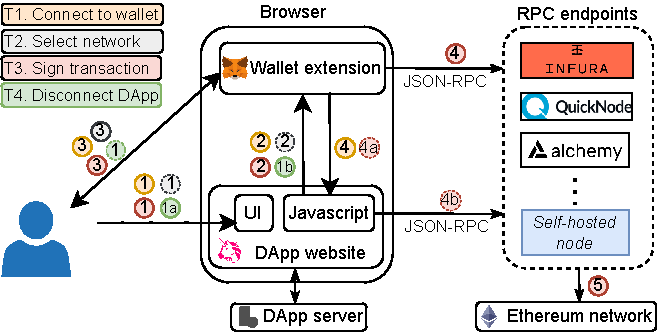
\includegraphics[width=0.47\textwidth]{web3-architecture.pdf}
    \caption{Overview of web3 architecture and user flow for four common tasks. 
    In T1, the user selects ``connect wallet'' on the DApp \protect\TONE{1} which requests the user's account address \protect\TONE{2}; the wallet obtains user approval \protect\TONE{3} and returns the address \protect\TONE{4}.
    In T2, the user selects a blockchain network on the DApp \protect\TTWODASHED{1} which triggers the wallet \protect\TTWODASHED{2} to prompt the user to switch network \protect\TTWO{3}; alternatively, the user can directly switch network on the wallet.
    In T3, the user initiates a transaction on the DApp \protect\TTHREE{1} which sends it to the wallet \protect\TTHREE{2}; the wallet prompts the user for approval \protect\TTHREE{3} and if approved, the wallet sends its proof to an Ethereum node via JSON-RPC APIs \protect\TTHREE{4} which is then broadcast to the Ethereum network \protect\TTHREE{5}; alternatively, the proofs could be routed through the DApp \protect\TTHREEDASHED{4a} before reaching the network \protect\TTHREEDASHED{4b}.
    In T4, the user selects ``disconnect wallet'' on the DApp \protect\TFOUR{1} which asks the wallet to revoke its permissions \protect\TFOUR{2}; alternatively, the user can directly disconnect on the wallet \protect\TFOURDASHED{1}.}

    % using standard wallet API~\cite{providerAPI}
    
    % When a user connects their wallet to a DApp (1), the DApp's Javascript code sends a 
    % When the user initiates each task on the DApp, the DApp's code sends a request to the wallet using standard APIs~\cite{providerAPI} (\textit{eth\_requestAccounts} and \textit{eth\_sendTransaction}) or wallet-specifc
    % uses the \textit{Ethereum Provider API}~\cite{providerAPI} to
    \label{figWeb3Architecture}
\end{figure}

\subsection{RPC endpoints}
% DApps offer services on different \ac*{EVM} chains, thus requiring users to connect to different chain networks.
DApps and wallets rely on RPC endpoints\footnote{\url{https://rpc.info/}} to exchange transaction data with \ac*{EVM} networks, using the standard JSON-RPC API~\cite{metamaskJsonRpcApi}.
For instance, MetaMask relies on Infura as its default endpoint~\cite{metamaskInfura}; note that these separate services are both owned by the same entity.
% These networks involve Web3 middleware providers 
% Network providers of these middleware servers
These endpoints relate to different privacy implications, e.g., some providers maintain logs of user data transmitted through their servers while others state that they do not collect any user data.
Thus, it is important for users to choose endpoints that align with their privacy preferences.

\section{Related work}
% Many previous studies have explored security risks and usability of individual applications.

The usability literature has explored Bitcoin~\cite{eskandari2018first,gao2016of,krombholz2017the,mai2020user,sas2017design} and generic blockchain technology~\cite{frohlich2022blockchain,jang2022userExperience,jang2020userPerspectives}. In terms of Ethereum, web3, and wallets such as MetaMask, the literature has focused on user perceptions. 
Panicker et al.~\cite{panicker2024end} found that users do not fully comprehend risks involved in token transfers in MetaMask UIs due to a lack of information about outcomes.
Analyzing app reviews of mobile wallets, Voskobojnikov et al.~\cite{voskobojnikov2021u} observed misinformed mental models due to an overreliance on understanding of traditional web 2.0 systems.
Si et al.~\cite{si2024understanding} explored user interactions and risk perceptions across the Web3 ecosystem, finding user concerns about vulnerable contracts and social engineering attacks involving inadvertent approvals.
By contrast, our study learns through direct interaction with a broad set of popular DApps `in the wild.'
% Usability studies:
% - usability testing of a single DApp~\cite{jang2020userPerspectives};
% - evaluation framework for user study of blockchain systems~\cite{jang2022userExperience};

% User awareness/concerns:
% - user awareness of transfer risks~\cite{panicker2024end};
% - risks perceived by users in Web3~\cite{si2024understanding};
% - analysis of wallet app reviews shows overreliance on traditional banking systems~\cite{voskobojnikov2021u};

% proposals to improve contracts:
% - automated generation of user notices~\cite{hu2021automating};
% - authentication information/warnings about contracts~\cite{gallersdorfer2021augmenting};


% General blockchain:
% - user mental models of cryptocurrency systems~\cite{mai2020user};
% - SoK of HCI papers of blockchains, role of trust was the top theme~\cite{frohlich2022blockchain};

% the user doesn't care whether it's MM or app (either is a usability issue. which happen to be MM) -- the paper is about usability issues when user use Web3/make transactions

% spreadsheet -- work, contributions, how our paper is different;

\section{Methodology}

A cognitive walkthrough~\cite{wharton1994cognitive} is a usability evaluation methodology often employed first to establish a priority list of usability issues to be considered with other methods. A dual expert (knowledgeable in both usability and in the domain of study---web3, in our case) evaluates if users with a specific persona (\textit{e.g.,} no prior familiarity) can successfully use an application interface and complete a set of core tasks without violating a set of guidelines.
For our study, we assume that users are comfortable with web 2.0 websites and browser extensions.
We also assume basic familiarity with blockchain user interfaces, e.g., gained from bitcoin wallets that have existed before web3 DApps.
Two evaluators independently generated an initial list of tasks users perform on web3 DApps. Then we discussed each task and whether a similar task has been studied in the past (\textit{e.g.,} as part of bitcoin wallet evaluation) and agreed to focus on tasks unique to web3.
We excluded one-time tasks (such as setting up an Ethereum wallet) and decided to focus on frequent tasks users need to perform across DApps.
Our final list of core tasks included:

\begin{enumerate}
    \item [T1.] Connect MetaMask wallet to a given DApp website. %preferred wallet (MetaMask) to a given DApp website.
    \item [T2.] Configure wallet to connect to a desired blockchain network (if it is not already on it). This network has to be supported by the DApp to perform transactions; the supported networks may be different on each DApp. %supported by the DApp; this may be different on each DApp depending on the network on which it is built. 
    \item [T3.] Conduct an operation of the DApp site that does require wallet approval, configure and sign the transaction, understand and avoid risks. Covers token balances, gas fees, approvals, signature, confirming transaction, etc. %Approve transactions by signing token transfer requests from their wallet to the DApp's contract.
	\item [T4.] Revert, to the extent possible, any past interactions with the DApp including disconnecting the wallet and revoking permissions.
\end{enumerate}

Fig.~\ref{figWeb3Architecture} shows the workflow of these tasks.
We perform walkthroughs by simulating step-by-step user actions in each core task and asking ourselves whether the interface satisfied a list of usability guidelines.
We draw our guidelines directly from the established usable security literature---specifically past studies of Bitcoin~\cite{eskandari2018first,moniruzzaman2020examining}. We repeat verbatim:

\begin{enumerate}
    \item[G1.] Users should be aware of the steps they have to perform to complete a core task.
    \item[G2.] Users should be able to determine how to perform these steps. % recognizability of steps to complete task
    \item[G3.] Users should know when they have successfully completed a core task. % visibility of system status
    \item[G4.] Users should be able to recognize, diagnose, and recover from non-critical errors. % provide users control
    \item[G5.] Users should not make dangerous errors from which they cannot recover. % prevent dangerous errors
    \item[G6.] Users should be comfortable with the terminology used in any interface dialogues or documentation.
    \item[G7.] Users should be sufficiently comfortable with the interface to continue using it.
    \item[G8.] Users should be aware of the application’s status at all times. % keep users informed
\end{enumerate}

A walkthrough allows for an evaluation across a large number of DApps, in contrast to time-limited and costly user studies. During initial analysis, the two evaluators performed walkthroughs on different DApps to identify problematic areas and inform further walkthroughs.
%discussed the walkthrough procedure for two popular DApps (ENS and Uniswap). 
%We settled on the above three core tasks because these are primary tasks that reflect typical user workflows of interaction with DApps and contracts.
%If users are not fully informed during these core tasks, attackers can mislead users into granting access to their wallet data and assets.
%For each core task, we analyzed the information displayed to users and evaluated if each interface satisfied the above guidelines, taking note of violations. 
After refinement based on this analysis, the main researcher evaluated each of the top 50 DApps listed on \textit{DAppRadar},\footnote{\url{https://dappradar.com/}} ranked by the total value of assets held under the DApp's contract over a 30-day period (Nov 2024). We used the MetaMask wallet for these tasks.
%This list allows us to focus on the most popular Web3 services and identify opportunities for improvements.



%We used the Cognitive walkthrough evaluation framework~\cite{wharton1994cognitive} to evaluate the usability of Web3 transaction flows across 50 DApps in combination with the MetaMask wallet extension.
%Cognitive walkthrough is a task-based evaluation method where evaluators
% inspect the learnability of application UIs.
% The primary goal of the walkthrough is to 
%find if users with no prior familiarity (novice users) can successfully use an application interface and complete a set of core tasks.
% The first step in this method is to identify users' goals related to a set of core tasks and the steps involved in accomplishing the goals.
%To this end, the evaluators identify users' goals related to these tasks and follow the steps involved in accomplishing these goals.
%This method has been used in the blockchain context to identify issues in Bitcoin clients (cf.~\cite{eskandari2018first,moniruzzaman2020examining}).
%Herein, we evaluate DApp and wallet UIs involving more complicated flows compared to Bitcoin payments, such as connecting to different blockchains. % such as cross-chain transactions. 

%We chose cognitive walkthroughs because 
%they allow for evaluations across a large number of DApps (our evaluation cover three tasks on each of 50 DApps) compared to testing with actual users. % limits the number of DApps that can be evaluated.
% In addition, these evaluations provide early insights into the usability of new services such as Web3 DApps and wallets.
% In addition, the Web3 ecosystem is still new as there are only ~10M active users https://dappradar.com/blog/state-of-the-dapp-industry-q2-2024
%Our goal herein is to explicate common usability issues across popular DApp and wallet UIs that might lead to dangerous errors (such as losing funds by unknowingly approving malicious requests). %that are likely to impact Web3 users.
%To this end, the walkthroughs provide early insights on the usability of Web3 services and help us identify opportunities for improving security. %before broad adoption among users. 
% allow for identifying design issues in Web3 services before broad adoption among novice users.
% This type of evaluation is typically followed by usability testing of specific applications involving users.

%During initial analysis, two evaluators defined the core tasks and discussed walkthrough results of two popular DApps (ENS and Uniswap).
% This initial step helped refine our evaluation criteria for the remaining DApps.
%After refining our evaluation criteria based on this analysis, the main researcher evaluated each of the top 50 DApps listed on \textit{DAppRadar},\footnote{\url{https://dappradar.com/}} ranked by the total value of assets held under the smart contract over a 30-day period, as of Sept 2, 2024.
%This list allows us to focus on the most popular Web3 services and identify opportunities for improvements. %to evaluate the usability of connecting wallets, selecting networks, and approving transactions.

% \paragraph{Tasks.}
%For each DApp, our walkthroughs involved performing a set of three typical tasks users need to complete when making transactions in Web3 services:
%\begin{enumerate}
%    \item [T1.] Connect preferred wallet (typically installed as a browser extension) to a given DApp website.
%    \item [T2.] Configure wallet to connect to a specific blockchain network (if it is not already on this network) supported by the DApp; this may be %different on each DApp depending on the network on which it is built. 
    % The DApp can automatically trigger a wallet prompt to make this switch, although it is the user's responsibility to verify the legitimacy of the specific blockchain.
%    \item [T3.] Approve transactions by signing token transfer requests from their wallet to the DApp's contract.
%\end{enumerate}



% \paragraph{Guidelines.}
%\noindent
%For our walkthroughs, we compared the interfaces against a set of usability guidelines used in previous walkthroughs~\cite{eskandari2018first,moniruzzaman2020examining}.
%Using guidelines is an effective approach common in many expert evaluation methods (e.g., heuristic evaluations~\cite{nielsen1992finding}, guideline reviews~\cite{bastien1995evaluating}).
% used a standard set of usability guidelines 
% derived from heuristic evaluation~\cite{nielsen1992finding}, a more general evaluation method often combined with cognitive walkthroughs. In heuristic evaluations, the evaluator, who is a dual expert proficient in usability best practices and in the domain of the evaluated application, compares the evaluated system against a set of usability guidelines.
%We used the specific set of guidelines from~\cite{eskandari2018first}:
%\begin{enumerate}
%    \item[G1.] Users should be aware of the steps they have to perform to complete a core task.
%    \item[G2.] Users should be able to determine how to perform these steps. % recognizability of steps to complete task
%    \item[G3.] Users should know when they have successfully completed a core task. % visibility of system status
%    \item[G4.] Users should be able to recognize, diagnose, and recover from non-critical errors. % provide users control
%    \item[G5.] Users should not make dangerous errors from which they cannot recover. % prevent dangerous errors
%    \item[G6.] Users should be comfortable with the terminology used in any interface dialogues or documentation.
%    \item[G7.] Users should be sufficiently comfortable with the interface to continue using it.
%    \item[G8.] Users should be aware of the application’s status at all times. % keep users informed
%\end{enumerate}

\subsection{A Sample Walkthrough}

For space considerations, we do not present the full details of each walkthrough of 3 tasks over 50 DApps. Instead, we present one representative sample walkthrough to illustrate what the methodology looks like, and then we present our overall results, based on all walkthroughs, in the next section.
The sample is the (T3) transaction approval task in the DApp Uniswap~\cite{uniswap}, a decentralized exchange service on Ethereum allowing users to exchange one type of (ERC-20) token for another.
We assume the persona of a typical web3 user who owns one or more tokens, uses a common wallet such as MetaMask, and has basic understanding about Ethereum tokens and transactions.
For this task, we also assume the user has already connected their wallet to Uniswap (T1) and successfully switched to a target network (T2). % exchange ETH to Tether USD on Base

The swap page on Uniswap site prompts the user to select the tokens and the exchange amounts.
After selecting a token (ETH) to sell, the prompt shows the available wallet balance and an option to use the maximum amount. We input an arbitrary amount to sell,
% The dropdown option to select token for buying displays a long list of tokens.
and select to buy USDT using the token search option.
% If the input is a variation of the token (e.g., ``usdt''), the search returns an empty list.
% This is a slight violation of G1.
The search displayed the correct token only when the input exactly matched ``USDT''. Other variations (e.g., ``usdt'' or ``tether'') did not yield similar results, violating G1.
The results included two tokens displayed with the same name ``Tether USD'' and symbol ``USDT'', though with different icons and addresses.
% potentially confusing users despite differences in the address. %, and a warning icon beside one of the result. 
% This could confuse users despite the token addresses are different. 
Selecting any of the two tokens prompted a warning stating that the token is not popular among past transactions, however only one of the token included a warning icon.
Although these warnings aim to alert users about potential scams, conflicting cues likely cause confusion and reduce the effectiveness of warnings.
% Then, a prompt is shown to confirm swap along with estimated fees.

Uniswap triggers a wallet prompt with details about the transaction. %and prompts for user approval.
At the top of the prompt, a small icon beside the contract address displays a generic message prompting users to verify before trusting the contract.
This violates G2 as there is no guidance on how to verify.
The prompt also includes a section with predictions about the resulting balance changes, however this is not guaranteed as indicated within an icon.
We discuss this issue further in Sec.~\ref{sec:results:contracts}.
The prompt also includes estimated gas fees and an option to set a limit on the maximum fee.
This option (in a new prompt) lists four choices with different limits and processing times (options with lower fees tradeoff on longer wait times).

After selecting ``low'' gas and submitting the transaction,
the wallet notified that the transaction had failed without any description of the issue.
An external link from the wallet showed the error output directly from the contract, however this message is ambiguous with no instructions on recovery options.
This violates G4.
% failed txn -- https://basescan.org/tx/0x6179f9c2c2a502c21199df313b4e221cb9bc3b7c37eed1c828e9ebaaf9e603f4
% The notification led to a wallet prompt which also did not state the issue and only included an external link for details about the status.
Uniswap's troubleshooting guide~\cite{uniswapTransactionFail} lists potential reasons for transaction failures including possible issues caused by low gas limits, although users cannot be expected to find such resources for each transaction failure.\footnote{We attempted another transaction submitting with the default (``market'') gas fee limit, which was successful.}
The DApp/wallet interface can address these issues by explaining transaction failures and providing instructions on possible recovery options.

% described the status as \texttt{Fail with Custom Error 'TransactionDeadlinePassed ()'}; without any further instructions, this may not be sufficient to help users identify and recover from the issue (violating G4).\footnote{Uniswap had set a 10-minute limit on transaction wait times; Lowering the gas fee limit on MetaMask led to the transaction to wait past this deadline, and thus triggering the issue. See~\cite{uniswapTransactionFail} for further details. The DApp/wallet interface can help users by describing the issue and providing instructions on possible recovery options.} 
% We set a lower limit for gas fees since users might prioritize paying less for gas (trading off on longer transaction wait times).

%We set a lower limit for gas fees since users might prioritize paying less for gas (trading off on longer transaction wait times).

% the prompt does not provide information about risks 

\subsection{Limitations}
Our findings cover 50 popular DApps with MetaMask which may not be representative of other DApps and wallets.
We also do not cover mobile wallets and DApps accessed through mobile browsers. % involved wallets and DApps used on a desktop web browser.  
We evaluated a set of three core tasks which does not cover other tasks users might perform on DApps, such as connecting with other users on social DApps.
% For example, users may use DApps to connect with other users in web3 games.
Finally, our expert evaluations may not accurately represent users' behavior in practice. % uncover all usability issues faced by typical users.
Our evaluations still uncover important usability issues that carry significant security and privacy implications for users.
% this first look usability evaluation aims to identify high-priority
% We particularly focused on violations that may lead to dangerous errors (G5) that likely carry significant security and privacy implications.
% In Section~\ref{sec:results:topIssues}, we discuss the violations that may lead to dangerous errors (G5) with significant implications to security and privacy.


%differentiated only by icon, token address and a warning icon on one result.
% Though the differences are not prominent, the warning aligns with G5 by suggesting that the token is not popular and thus may be a scam. %informing that the token is not frequently swapped.
% The warning suggests that the token is not popular and thus may not be trustworthy (G5).




%%% BEGIN OLD VERSION
% In the first step of our walkthrough of T3 (transaction approval for token exchange), we specified an arbitrary amount of 0.05 ETH to swap for ARB tokens on Uniswap's swap web page.
% % The settings dropdown option in this page indicates the default \textit{transaction deadline} as 10 minutes; note that if a transaction reaches this deadline before succeeding, the chain is \textit{reverted}~\cite{alchemyRevertTransaction} back to the original state.
% Next, we submitted the swap request which triggered a MetaMask extension prompt showing the token amounts to exchange along with estimated gas fees and an option to set a limit on the maximum fee. %the user is willing to pay %; Lower fee limits trade off transaction wait times for lower gas cost.
% We set a lower limit for gas fees since users might prioritize paying less for gas (trading off on longer transaction wait times).
% % cause longer transaction wait times as nodes might prioritize higher value transactions.
% % If gas fees in the network are above this maximum value, the transaction
% We submitted the transaction. 

% After a few minutes, the wallet showed a browser notification that the transaction had failed without any information about the cause.
% The notification led to a wallet prompt which also did not state the issue and only included an external link for details about the status.
% This page described the status as \texttt{Fail with Custom Error 'TransactionDeadlinePassed ()'}; without any further instructions, this may not be sufficient to help users identify and recover from the issue (violating G4).\footnote{Uniswap had set a 10-minute limit on transaction wait times; Lowering the gas fee limit on MetaMask led to the transaction to wait past this deadline, and thus triggering the issue. See~\cite{uniswapTransactionFail} for further details. The DApp/wallet interface can help users by describing the issue and providing instructions on possible recovery options.} 
%%% END OLD VERSION


% our focus isn't on which wallet is more usable (or specific wording) but the goal is to the provide an overview of the main issues;

% we found many issues, but there were four main themes

% = = = = = = = = = = = = = = = = = =  = = = = = = = = =

\section{High Priority Usability Issues}
\label{sec:results:topIssues}

We now present the highest priority issues we found during our walkthroughs of 50 DApps, focusing on issues that may lead users to make dangerous errors (G5). We would direct future research efforts to consider these issues.

%that may lead users to make dangerous errors. % related to the user interface design identified during our walkthrough of the tasks.
%We focus on issues that may lead users to make dangerous errors (G5). 
% We now describe the common issues identified during our walkthrough of the tasks and discuss potential improvements to reduce risk of attacks.

% TODO -- one or two sentences that this section of all the dangerous errors we found

% TODO -- Describe identified issues along with usability best practices, list out wallet security indicators and suggest improvements

% = = = = = = = = = = = = = = = = = =  = = = = = = = = =

\subsection{Issue 1: Weak link between wallet prompts and DApps}

Users can have multiple DApp websites open at once, while the wallet is a singular and separate interface. We found MetaMask attempts to associate prompts with its originating DApp by displaying domain names, however it is inconsistent. In some cases, it does not link prompts to websites: \textit{e.g.,} `allow \textit{this site} to add a network?' Connecting to a malicious network compromises the user's privacy (links user's IP address and wallet addresses), displays information about the state of the blockchain, and can propose fraudulent transactions (timed to follow specific user actions). In other cases, the domain is shown but the visual cue varies (boxed/rounded/unboxed; domain/url/favicon; sizes/colors/locations). 

Transactions can also queue, say if a user forgets to sign/cancel a transaction in MetaMask or clicks multiple times on the website. MetaMask indicates the number of current requests in the extension icon and a textual indicator in a small font size, but is easy to miss. Users, who have unknowingly queued a transaction and proceed to a new DApp where they take an action that creates a transaction, will be presented with the earlier queued transaction for signature first. 



%Many wallet permission prompts do not include visible cues to link the displayed prompt to the requesting DApp. For example, when the user is prompted to change the blockchain network on MetaMask, the permission prompt displayed by MetaMask does not indicate which DApp triggered this request.
%The lack of a standard interface design connecting permission prompts to the requesting site increases the likelihood that users inadvertently approve requests by malicious actors (e.g., changing to a network controlled by an attacker). 
% explain risk of adding custom networks
%Simply connecting to a malicious network compromises the user's privacy as the network can record the user's IP address and link it to their wallet addresses.
%Connecting to malicious networks also allows attackers to display false information about the state of the blockchain such as incorrect balances and fraudulent transactions.

%The issue becomes exacerbated when users interact with multiple DApps in parallel. In this scenario, say a user initiates a first transaction on a DApp (e.g., to swap tokens on an exchange DApp) which would involve multiple wallet prompts (to connect wallet to DApp, to choose network from which tokens need to be swapped, and to approve transfer to the DApp's contract).
%Before completing these steps, the user visits another DApp and initiates a second transaction. 
%When the new transaction request is received by the wallet, the wallet re-displays the prompts related to the previous transaction, although users may incorrectly assume the prompts as related to the current transaction.
%this forces the user to complete (or reject) it before displaying the new transaction.
%Although MetaMask indicates the number of current requests in the extension icon, the design raises concerns about possible confusion between the user's assumption about the requesting DApp and the actual DApp being granted approval.

\subsubsection*{\textbf{Recommendation}}
%Standard usable security guidelines~\cite{whitten1999johnny,clark2007usability} suggest interface design that prevents users from making dangerous errors.
%Thus in the context of DApps, it is important for users to easily associate wallet prompts to the originating DApp.
A previous paper~\cite{gallersdorfer2021augmenting} introduces TLS-based authentication of contracts and proposes augmenting MetaMask interface with warnings (similar to web 2.0 browser certificates), though MetaMask has not included such proposals.
We recommend that the requesting DApp's URL is in every wallet prompt in a standard format (i.e., location in the UI) across all DApps.
The wallet could also warn users when the requesting DApp is not in the current (in-focus) view, bring the requesting DApp's web page to in-focus view, or disable the approve button until the page is in focus to limit inadvertent approvals.
%, e.g., by highlighting the mismatching URL in red font and offering an option to bring the requesting DApp's web page to in-focus view.
% display prompts along with the web page that triggered the prompt by moving the window to in-focus view;
%For certain DApps (such as those unverified by the wallet or visited by the user for the first time), the wallet could restrict approval 
%by disabling the approve button until the page is in focus to limit inadvertent approvals.

% = = = = = = = = = = = = = = = = = =  = = = = = = = = =

\subsection{Issue 2: Cross-chain switching issues}
It is a common task for users to switch their wallet to different networks when interacting with DApps.
% When switching to a network unrecognized by MetaMask, the wallet prompt includes multiple warning messages about the unverified network; these messages are not included for a subset of the major networks recognized by MetaMask.
When adding a new network to the wallet, it is the user's responsibility to evaluate its security and privacy as MetaMask does not verify. % the legitimacy of networks. 
However, this tends to be an arbitrary process where users need to rely on ad-hoc web searches to check the network~\cite{metamaskVerifyNetwork}.
%This hapahazard approach is also problematic because it requires the user to move away from their current task of adding a network and making transactions.
This manual process is also extensive as it involves verifying the individual details displayed about the network including the network's name, \ac*{RPC} URL, chain ID and its currency.
% Side note: there may be instances where a chainID is reused (e.g., deprecated chains)

% Choosing an \ac*{RPC} provider is important since each provider offers different security and privacy benefits.
There are three options for adding a new network on a MetaMask wallet, and each option may involve different privacy and security implications:
\begin{enumerate}
    \item Users may add a new network from a DApp site (e.g., by initiating a transaction on the relevant blockchain) which would send the wallet information about the network including the DApp's preferred \ac*{RPC} URL. In this case, the wallet simply displays this information and prompts the user to add the network. This prompt does not allow the user to select a different (e.g., more privacy-friendly) \ac*{RPC} provider, or even indicate the possibility of changing providers. Thus, users may consent to using the displayed network though they may not be fully informed or even aware of more privacy-friendly choices. %If the user approves, it is assumed that they have consented (although they may not be fully informed) to the provider's privacy policies. 

    \item Second, for a subset of (popular) networks, users can add the network automatically from the wallet interface using network details pre-filled by the wallet. %; the UI in this option warns about privacy issues in networks that include tracking.
    Wallets may be able to inform users about potential security and privacy issues with these providers, however, this may be possible only for a limited number of networks. %and unlikely to cover all network providers.

    \item Third, users can add a network on their wallet by manually entering all the network details including their preferred \ac*{RPC} provider. Although this option offers the most control to users, it may not be straightforward to identify legitimate network providers that are secure and private.
\end{enumerate}

These issues complicate the process of adding networks to the wallet by requiring users to perform multiple out-of-band checks (i.e., breaks the user's workflow for the task by involving external resources and ad-hoc web searches).
MetaMask prompts include multiple warnings when any the network information (e.g., name, RPC URL, or currency) provided by the DApp do not match its own records.
However, users may become desensitized to security warnings especially when they are frequently linked to false alarms~\cite{krol2012Dont}.
% Asking users to re-validate information about networks already in their wallet and showing excessive number of warnings (e.g., when a DApp uses a different network name despite not affecting security) may lead 
% Users may become desensitized to frequent security warnings and false alarms, as found in previous studies on security indicators in Web2 apps (e.g.,~\cite{krol2012Dont}).
% In web3, the current wallet design of prompting users to re-add blockchains and showing excessive number of warnings may be ineffective.

\subsubsection*{\textbf{Recommendation}}
When adding a network, users should be made aware of alternative providers who may offer better security and privacy.
To this end, when adding networks via DApps, wallets can simply display an option to change the provider before adding to the wallet.
It is important for users to be informed about available choices before they make a decision since adding a network to the wallet immediately exposes personal information such as user's IP address and wallet addresses (which can then be linked to past transactions, compromising privacy).
To further support informed user decisions, DApps and wallets could list more than one provider for the user to choose from, and provide information about the benefits of each network in terms of speed of transactions, gas fees, security and privacy properties; existing resources such as ChainList\footnote{\url{https://chainlist.org/?chain=1}} already provide information about alterantive \ac*{RPC} servers and their privacy and speed.

% To support informed user choices about networks, DApps and wallets should provide information on security and privacy policies of network providers.
% This approach would involve fewer user checks and thus may reduce user fatigue.
% The number of false warnings can be reduced if the wallet prompts

% = = = = = = = = = = = = = = = = = =  = = = = = = = = =

\subsection{Issue 3: Unpredictable function behaviour}
\label{sec:results:contracts}
% TODO -- look into ASE 2021 (Automating user notice generation for smart contract functions) https://ink.library.smu.edu.sg/cgi/viewcontent.cgi?article=7840&context=sis_research
% Issues -- Contracts are difficult to verify, e.g., not enough information on prompts to help users verify; unverified contracts are noticeable (wallet just shows the hex values for unverified addresses)
% Similar to any unknown code, 
%There are several risks associated with contracts, including potential for loss of the user's funds due to vulnerabilities and scams.
% It is important to provide users with information about the contracts they interact with to help mitigate these risks.
% However, users are not provided with information about contracts to inform about these risks.
%During our analysis, we observed interfaces to be often lacking useful information about the risks of triggering contracts. %with partially useful information about contracts, however these were often incomplete or limited to certain transactions.
When prompting for a transaction approval, MetaMask includes predicted changes to the user's balances (i.e., the amount ``sent'' and amount ``received'') for recognized tokens and blockchains~\cite{metamaskEstimatedChanges}.
% This feature~\cite{metamaskEstimatedChanges} involves sending transaction data to the wallet's server, which raises privacy concerns.
% In addition to accuracy concerns, 
% These predictions might lead to misplaced trust on DApps as some users might falsely believe that they would be receiving tokens, i.e.,  
These predictions may mislead users into falsely assuming that running the contract would actually result in receiving tokens whereas the wallet does not perform any security checks, i.e., misplacing trust on the contract despite the lack of validation and security checks.
Though the wallet warns (in a small icon) that the predictions are not guaranteed, users may not fully comprehend the risks or miss the warning completely.
% TODO -- find usable security work related to trustworthness. E.g., https://www.sciencedirect.com/science/article/pii/S1071581905000121

% These predictions might lead to users misplacing their trust on the contract despite the lack of any security checks by the wallet.
% lead to misplaced trust on the contract as some users might believe that the ``receive tokens'' amount as

% MetaMask transaction prompts include estimated changes 
% MetaMask prompts that included potentially useful information showing the estimated changes to the user's wallet
% with partially useful information about contracts, 
% MetaMask offered useful information for a limited number of contracts, 
% however such information was limited to certain tokens and contracts.

Other approaches have been proposed to extract information about contracts.
Solidity, the primary language for contracts, provides developers the ability to write special user-facing comments about their contract code~\cite{solidityNatspec}.
However, most of the contracts in the wild do not include such comments~\cite{hu2021automating}.
Automated generation of these comments could help fill this gap~\cite{hu2021automating} but such comments may not provide accurate descriptions of contracts and may lead some users into a false sense of security.
Another line of research focuses on security tools (e.g.,~\cite{kalra2018zeus,tsankov2018security}) to identify vulnerable contracts, however informing users about these issues (e.g., in end-user interfaces) remains an open challenge.

% Although there are proposals and implementations that could help inform, we observe a lack of standard design that 


% what can the wallet tell you about a transaction to help you avoid dangerous transactions (fundamental limitation, like buyer beware)

% static analysis could help but it's not bulletproof
% OPTION1: there is a privacy tradeoff, but good first step but there's room for way more
% OPTION2: better to do nothing because if might give a false sense of security 

% Recommendation -- Unverified contracts should be more prominent (e.g., using different color); use of allow lists?; other proposed solutions
\subsubsection*{\textbf{Recommendation}}
% It is important for wallet interfaces to inform users about contracts before they approve transactions.
Wallets should use a standard interface design to inform users about contract risks.
When interfaces includes predictions about balance changes, it should clearly warn users about the lack of validation about the DApp to limit false trust assumptions.
All warnings should be displayed using a standard and prominent format.
Future research can determine the extent to which malicious behaviour can be predicted through automated analysis (or DApps could default to untrusted until certified). 

% = = = = = = = = = = = = = = = = = =  = = = = = = = = =

\subsection{Issue 4: Concerns with \textit{Allowance} mechanism}
% look into RAID 2022 paper https://dl.acm.org/doi/pdf/10.1145/3545948.3545963
%- unlimited approval is prevalent (based on public transactions data), likely due to many DApps requesting unlimited approval and not all wallets allow changing the amount.
%- unlimited approval involves big security risk since (1) the DApp may be malicious/hacked, and (2) the DApp may be honest but vulnerable contract may be exploited by attackers to steal approved funds
The final issue has been explored in the literature by Wang \textit{et al}~\cite{wang2022penny} but we include the issue for completeness.
Tokens deployed on Ethereum follow standard interfaces, such as ERC20, meaning wallet software can interoperate even without knowing anything specific about the token.
The ERC20 standard requires an `approve' function. Instead of Alice sending 10 tokens to Bob, she can approve Bob to take 10 tokens from her at any time until she removes the approval. 
Many DApps move tokens through approvals rather than transfers.
Prioritizing simplicity and flexibility over security,  60\% of DApps in \cite{wang2022penny} request \textit{unlimited} approvals. Unlimited approvals are problematic when a DApp is later compromised (or malicious to begin with)~\cite{incident2020Bancor,incident2021Primitive}.
Some DApps provide no option to adjust the approval amount, while some have been found to display one amount but prompt for unlimited (observed in \cite{wang2022penny} as an example of a deceptive/dark pattern~\cite{mathur2019dark}). While MetaMask does allow approvals to be adjusted, once set, it is up to the user to remember to un-approve.  

%(although other variants exist), 
%Many past incidents (e.g.,~\cite{incident2020Bancor,incident2021Primitive}) have revealed that the allowance mechanism of ERC20 tokens (i.e., allowing DApps %to spend user's tokens on their behalf) can be exploited to steal users' tokens.
%These incidents relate to the \textit{unlimited} approvals obtained by DApps which are malicious or are benign but vulnerable.
%In our study, all approval requests by DApps triggered wallet prompts displaying unlimited allowance amounts. 

%A recent analysis~\cite{wang2022penny} of approval transactions made by users revealed that 60\% of these transactions were unlimited approvals.
%In addition, the study observed many DApp and wallet UIs which do not include an option to modify the approval amount.
%, increasing the risk of inadvertent approvals without limits.
%The study also found two misleading instances of DApps that displayed lower limits on their website but requested unlimited approval in the wallet prompt.
%We note that this type of misuse is a form of deceptive pattern made possible by allowing DApps to specify the default approval amount displayed to users.
% In a form of deceptive pattern, DApps can trick users into granting higher approval limits.
% Based on our analysis, we note that using the approval amount specified by the DApp as the default value is not a safe design as DApps may trick users into granting higher approval limits using deceptive patterns.
%since this may prioritize the DApp over the best interest of users, allowing the use of deceptive patterns.
%Deceptive patterns are UI designs that trick users into making choices that may not be in their best interest such as tricking users to grant unlimited approvals.
%Such patterns have been observed in many Web2 sites, e.g., in shopping sites that design UIs to induce a sense of urgency to get users to spend more money~\cite{mathur2019dark}.
% common deceptive patterns found in Web2 applications design UIs to nudge users towards choices that may not be aligned in the interest of the user
% even when users can change the approval amount, it is 

% Issues -- Unsafe default as the spending cap is set by the DApp and is often set to max (unlimited) value.
% wallet shows this value and allows the user to change it, but it's not a safe default.

\subsubsection*{\textbf{Recommendation}}
Attention has been given to allowing users to view, modify, and revoke past approvals, both in the MetaMask dashboard and through third-party tools (e.g., \url{revoke.cash}~\cite{revokeCash}). Because of the ERC20 standard, wallets should recognize an unlimited approval and better warn users, schedule a reminder prompt to revoke for a later time, or allow users to set global limits (with sensible default values) on allowances.

%TWhile there is a lack of mechanisms to prevent users from making unsafe approvals, there exists options for users to reduce or fully revoke already approved allowances.
%MetaMask dashboard (separate from the transaction prompts) allow users to view and modify or revoke approvals, although such options may not be available on many wallets~\cite{wang2022penny}.
%There also exist tools besides wallets (e.g., \url{revoke.cash}~\cite{revokeCash}) that allow users to revoke approvals.
%While these tools are important and necessary, we recommend improving DApps and wallets to \textit{prevent} users from inadvertently granting unlimited allowances.
%For example, default spending limits should be set by wallets, accompanied by an option to use the amount requested by DApps; in addition, DApps can inform the user about benefits (e.g., intended savings on gas fees) of higher approval limits.
% Recommendation -- improve allowance mechanism so that user/wallet has more autonomy with spending caps (i.e., less control for the DApp). For example, wallet could enforce more moderate defaults based on user's preferences or past transaction amounts.


% \section{Research Agenda}
% result of this paper is that usability is a big concern; important to fix this; so our contribution is which areas to focus on to improve usable security; Future work would likely involve a user study;

% (for writing -- see example papers on usability on other areas such as bitcoin)

% new field (but many issues are similar to earlier web); these issues need to be sorted out as it moves towards mass adoption; necessary first step to discuss shortcomings;







% \begin{credits}
% \subsubsection{\ackname} A bold run-in heading in small font size at the end of the paper is
% used for general acknowledgments, for example: This study was funded
% by X (grant number Y).

% \subsubsection{\discintname}
% It is now necessary to declare any competing interests or to specifically
% state that the authors have no competing interests. Please place the
% statement with a bold run-in heading in small font size beneath the
% (optional) acknowledgments\footnote{If EquinOCS, our proceedings submission
% system, is used, then the disclaimer can be provided directly in the system.},
% for example: The authors have no competing interests to declare that are
% relevant to the content of this article. Or: Author A has received research
% grants from Company W. Author B has received a speaker honorarium from
% Company X and owns stock in Company Y. Author C is a member of committee Z.
% \end{credits}
%
% ---- Bibliography ----
%
% BibTeX users should specify bibliography style 'splncs04'.
% References will then be sorted and formatted in the correct style.
%
\bibliographystyle{IEEEtran}
\bibliography{bib}
%
% \begin{thebibliography}{8}
% \bibitem{ref_article1}
% Author, F.: Article title. Journal \textbf{2}(5), 99--110 (2016)

% \bibitem{ref_lncs1}
% Author, F., Author, S.: Title of a proceedings paper. In: Editor,
% F., Editor, S. (eds.) CONFERENCE 2016, LNCS, vol. 9999, pp. 1--13.
% Springer, Heidelberg (2016). \doi{10.10007/1234567890}

% \bibitem{ref_book1}
% Author, F., Author, S., Author, T.: Book title. 2nd edn. Publisher,
% Location (1999)

% \bibitem{ref_proc1}
% Author, A.-B.: Contribution title. In: 9th International Proceedings
% on Proceedings, pp. 1--2. Publisher, Location (2010)

% \bibitem{ref_url1}
% LNCS Homepage, \url{http://www.springer.com/lncs}, last accessed 2023/10/25
% \end{thebibliography}
\end{document}
